%% content.tex
%%


\chapter{Einleitung}
\label{ch:Introduction}
%motivation.
Warum sind Schatten in der Computer Grafik eigentlich so wichtig?
Schatten geben nicht nur besser aussehende Bilder, sondern geben auch wichtige Informationen über Position und Skalierung von Objekte
(Abbildung \ref{fig:why-shadows}).

\begin{figure}[H]
	\begin{center}
		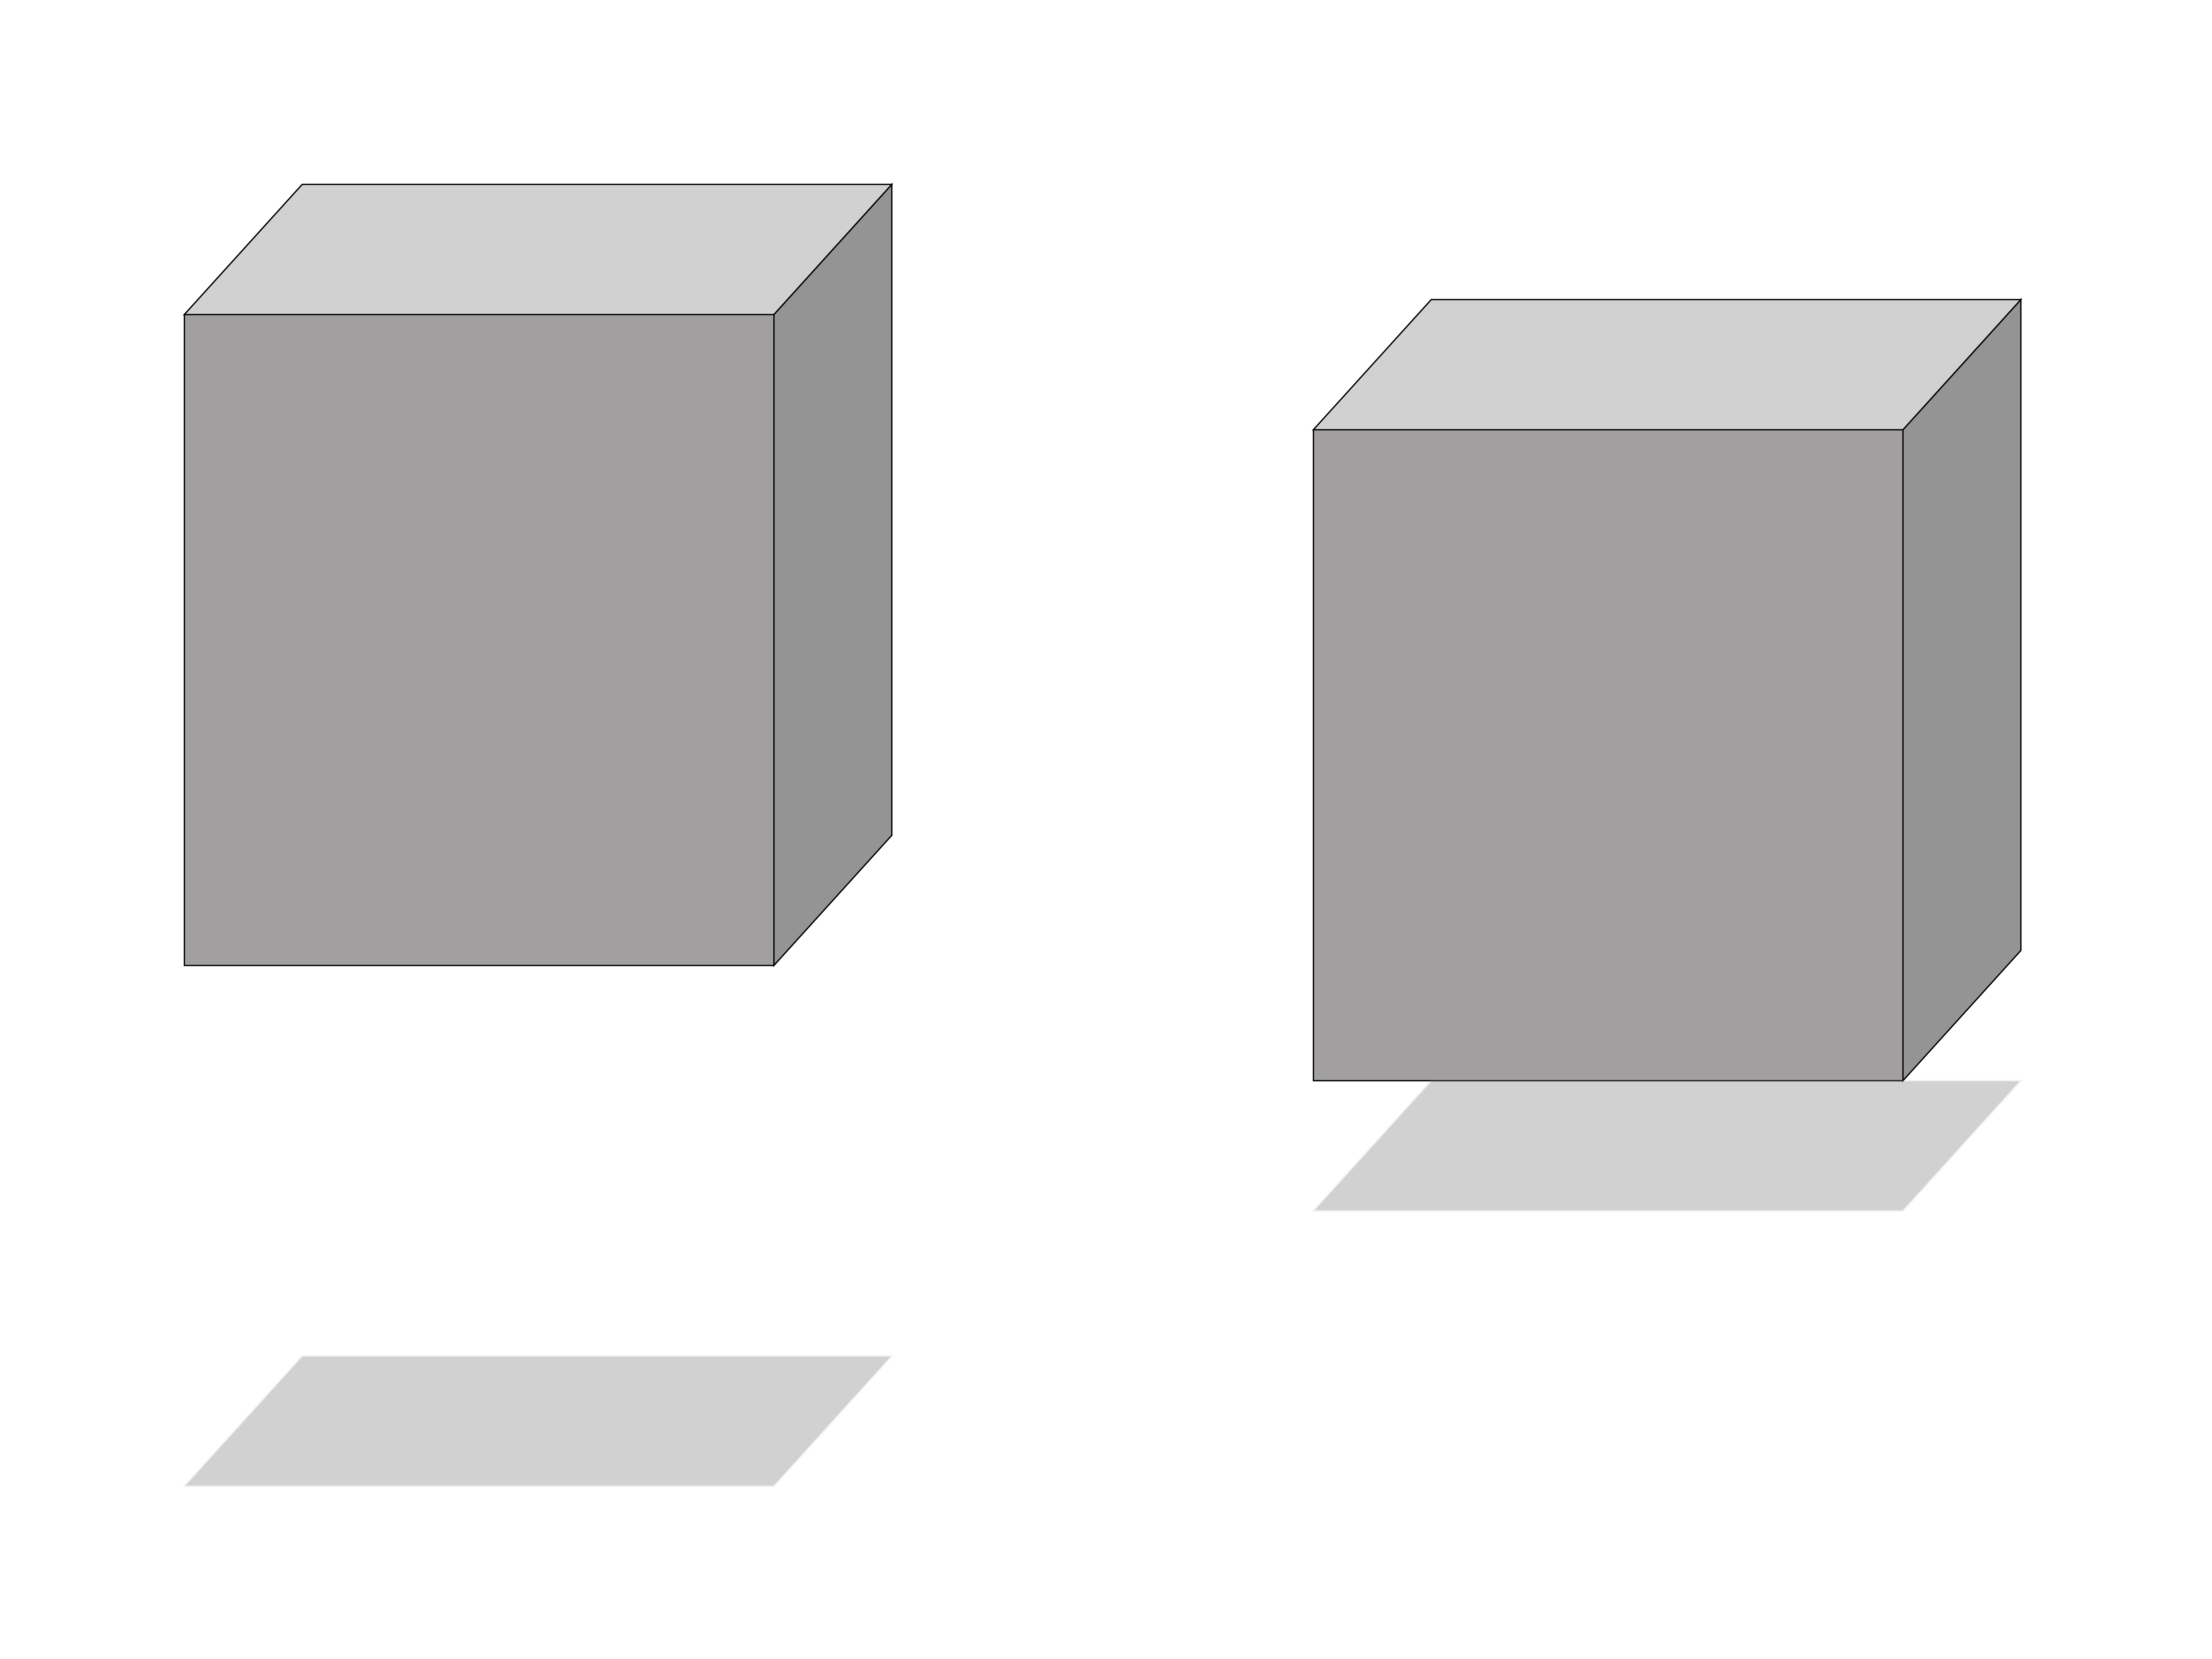
\includegraphics[width=.3\textwidth]{res/img/why-shadows.jpg}
    \caption{Es ist klar zu erkennen, das der linke Würfel höher über dem Boden schwebt als der rechte Würfel. 
    Ohne Schatten wäre es unmöglich zu entscheiden, welcher Würfel wieweit über dem Boden schwebt.}
	\end{center}
	\label{fig:why-shadows}
\end{figure}
%welches verfahren will ich vorstellen.
%Um den Schatten in einer Szene berechnen zu können muss zuhnächst für jeden Pixel bekannt sein, ob er im Schatten liegt.
%Dieses Problem scheint einfach. 
Ein Pixel liegt genau dann im Licht, wenn die Gerade zwischen Pixel 
und Lichtquelle von keinem anderen Objekte blockiert wird.
In einem Raytracing Renderer ist dies leicht umzusetzen. 
Um zu bestimmen, ob ein Punkt im Schatten liegt kann ein weiterer Ray von dem Oberflächenpunkt zu dem Licht berechnet werden, 
falls dieser ein Objekt schneidet so liegt der Punkt im Schatten.
Raytracing ist jedoch ein sehr aufwendiges Verfahren, deshalb wird in Echtzeitberechnungen von Bildern meistens
ein Rasterisierter Renderer verwendet.
In einem Rasterisierten Renderer ist es jedoch nicht möglich den Schnitt eines Rays mit der Szene
zu berechnen um zu bestimmen, ob ein Punkt im Schatten liegt.
\newline 
\newline
Der bekannteste Algorithmus der Schatten in einer Rasterisierten Renderpipeline 
berechnet heißt Shadow Mapping.
In einem Raytracing Renderer wird für jeden Punkt berechnet, ob das Licht sichtbar ist.
Bei Shadow Mapping wird dies umformuliert. 
Ein Punkt liegt im Schatten, genau dann wenn der Punkt vom Licht sichtbar ist.
Dieses Verfahren kommt jedoch mit einigen Problemen, denn um zu berechnen, ob ein Punkt von dem Licht sichtbar ist,
wird die Szene aus der Perspektive des Lichtes auf eine Textur gezeichnet.
Dabei wird sich für jeden Pixel der Textur gespeichert wie, weit der nächstliegende Punkt von dem Licht entfernt ist.
Da es bei dem abspeichern zu einer Diskretisierung kommt rechnen 
wir in den Folgeschritten niemals mit der tatsächlichen Tiefe eines Punktes,
sondern mit einer Rundung zu dem nächstliegenden Diskretisierungswert.
Außerdem ist es durch die endliche Auflösung der Textur nicht möglich die Tiefenwerte eines exakten Punktes zu speichern,
sondern nur die Tiefenwerte eines Bereichs, der von einem Pixel auf der Textur beschrieben wird.
\newline
\newline
Trotz der vielen Probleme wird Shadow Mapping in vielen Echtzeit Applikationen verwendet.
Deshalb werde ich mit im weiteren mit dem Algorithmus auseinander setzen und dabei die Probleme die dabei auftreten untersuchen.
Dabei werde ich zunächst auf die Wert Diskretisierung in der Tiefen Textur eingehen.
Dies führt zu einem Artefakt, dass Selbstverschattung genannt wird, um dieses Artefakt zu verhindern gibt es 
viele Möglichkeiten ich will mich jedoch mit Heuristischen Biasing Methoden und Second Depth Shadow Mapping beschäftigen.
Anschließend werde ich auf Projektives und Perspektivisches Aliasing eingehen, diese Artefakte entstehen durch 
die limitierte Textur Auflösung der Shadow Map.
Um diese Artefakte zu beheben, gibt es eine überzahl an Verfahren, ich werde mich jedoch auf PSM, LiSPSM, CSM und PCF beschränken 
diese Verfahren bieten eine gute Grundlage für das Verständnis weiterer komplexerer Verfahren.
Am Ende will ich in einem Fazit eine Echtzeitfähige Kombination der vorgestellten Verfahren vorstellen.


% thematische einordnung (was auch immer has heißen soll)
% Kapitel gliederung erklären.

\chapter{Grundlagen der Rasterisierung}
\section{Koordinatensysteme}
\label{section:coords}
% hier wäre ein paar zitate schön die das ganze gut auf den punkt bringen.
Bei dem Rasterisierten Rendern zeichnen wir Objekte die aus Oberflächen (Dreiecken) bestehen.
Oberflächen bestehen aus Punkten die, die Position der Oberfläche relativ zu dem Objekt Mittelpunkt beschreiben.
Diese Koordinaten, die relativ zu dem Objekt geben sind, sind in einem Koordinatensystem, das \textbf{Object Space} heißt.
Um ein Objekt in der Welt verschieben zu können müssen alle Punkte eines Objekts (in Object Space) mit einer Linearen Transformation
in \textbf{World Space} transformiert werden.
Die Transformation besteht aus Skalierung, Translation und Rotation und wird meistens als 4x4 Matrix mit homogenen Koordinaten dargestellt.
Das Konzept einer Kamera lässt sich analog einführen.
Dabei werden alle Punkte im World Space mit einer Linearen Transformtion in \textbf{View Space} transformiert.
In View Space sind alle Punkte relativ zu der Kamera.
In einer weiteren Transformation wird nun die Art der Projektion der Kamera definiert. 
Dabei wird ein Punkt im View Space in \textbf{Clip Space} transformiert.
Die Transformation transformiert alle Punkte die sichtbar sind auf einen Punkt innerhalb eines Würfels der Größe 2x2x2 um den Ursprung.
Alle Oberflächen die außerhalb des Würfels liegen sind von der Kamera nicht sichtbar und werden nicht gezeichnet.
Aktuell haben wir nur Transformationen der Form $\mathbb{R}^3 \rightarrow \mathbb{R}^3$ betrachtet.
Um die Punkte auf dem Bildschirm darzustellen müssen wir eine Transformation der Form 
$\mathbb{R}^3 \rightarrow [0,1080]\times[0,1920]$ (Unter der Annahme, das der Bildschirm FullHD ist).
Diese Transformation wird von der Renderpipeline implizit durchgeführt, dabei werden alle Punkte in Clip Space 
auf die XY-Ebene projiziert und die Z-Werte werden als Tiefen Wert verwendet. 
Die Transformation transformiert somit Punkte von Clip Space in \textbf{Screen Space}.

\section{Projektion}
In Abschnitt \ref{section:coords} wurde bereits auf die einzelnen Koordinatensysteme und Transformationen eingegangen,
für die Kamera Projektion ist jedoch eine genaueres Verständis nötig.
Eine Kamera Projektion ist eine Abbildung von View Space in Clip Space.
Im Allgemeinen lassen sich alle Kamera Projektionen mit einem Frustum (Kegelstumpf) eindeutig charakterisieren.
Ein Kamera Frustum beschreibt einen Raum im View Space, 
der durch die Projektion auf einen Würfel im Clip Space abgebildet wird.
Eine Oberfläche des Frustums, die Near Plane, ist die Oberfläche auf die projiziert wird.
Die entgegengesetzte Oberfläche heißt Far Plane. 
Die Far Plane beschreibt die Punkte, die am weit möglichsten von der Kamera entfernt sind und noch sichtbar sind.
Insbesondere wird ein Gerade von einem Punkt auf der Near Plane zu einem entsprechenden Punkt auf der Far Plane
durch die Projektion auf eine Gerade projiziert die orthogonal zu der XY-Ebene liegt.
Dadurch wird klar, dass die Projektionstransformation, die Art der Projektion der Kamera definiert.
\newline
\newline
Projektionstransformationen werden oft mit einer $\mathbb{R}^{4\times{}4}$ Matrix implementiert.
Für eine orthogonale Projektion ist dies nicht nötig, da hier von $\mathbb{R}^3$ nach $\mathbb{R}^3$ abgebildet wird,
doch bei perspektivischen Projektionen wird die w-Komponente verwendet um die perspektive zu implementieren.
Dabei werden nach der Matrix Multiplikation die xyz-Komponenten durch die w-Komponente des Ergebnisvektors geteilt.
Dabei ist zu bemerkten, dass die z-Koordinate ebenfalls durch die w-Komponente geteilt wird. 
Dies ist im allgemeinen sinnvoll, den es führt zu einer nicht linearen Verteilung der Tiefe, wodurch die Tiefenauflösung
nahe bei der Kamera höher ist.

\section{Framebuffer}
Bei dem Zeichnen der Szene werden die Farb und Tiefenwerte der Pixel in einem Framebuffer gespeichert.
Dadurch das die Werte diskret gespeichert werden, enthält der Framebuffer nach dem rendern nicht die tatsächlichen Farb und 
Tiefenwerte, sondern eine Rundung auf den nächst gelegenen Werte.
Für die Farbwerte ist dieses Verhalten kein Problem, da der Unterschied zwischen 2 Farbwerten, die nebeneinander liegen, nicht erkennbar ist.
Dieses Verhalten führt jedoch bei Tiefenwerten dazu, dass die Tiefenwerte des Framebuffers niemals die tatsächliche Tiefe beschreiben.
Dieses Problem ist im Allgemeinen durch die nicht lineare Verteilung der Tiefenwerte, zwischen Near und Far Plane, kein Problem, 
doch im weiteren werden wir sehen, dass dies zu Problemen führt, wenn die Szene aus einer anderen Perspektive gezeichnet wird 
und die Ergebnisse in einem weiteren Zeichenschritt verwendet werden.

\chapter{Shadow Mapping} %that title blows.
\label{section:shadow-mapping}
Shadow Mapping \cite{Williams1978} ist ein Algorithmus zu Berechnung von Schatten 
in einer Rasterisierten Renderpipeline. 
Es ist das Verfahren, das in der Echtzeitberechnung am meisten zum Einsatz kommt, 
da es in einem Rasterisiertem Renderer implementierbar ist.
\newline \newline
Wie bereits in der Abschnitt \ref{ch:Introduction} erwähnt ist zur Berechnung von Schatten nötig, festzustellen,
ob ein anderes Objekt das Licht an einem Punkt blockiert.
Diese Berechnung für jeden Pixel direkt auszuführen ist in einem Rasterisiertem 
Renderer nicht möglich.
Beim Shadow Mapping Verfahren formulieren wir unsere Frage um und betrachten 
die Äquivalente Frage:
\textbf{Ist der Punkt von der Perspektive des Lichtes Sichtbar?}
Wenn ja dann wird das Licht von keinem Objekte blockiert.
Dieses umformulieren der Fragestellung hat den Vorteil das sie sich in
einem Rasterisierten Renderer berechnen lässt, indem die Szene aus der Perspektive des Lichtes gezeichnet wird.
\newline
\newline
\textbf{Der Shadow Mapping Algorithmus lässt sich in 2 Schritte 
unterteilen:}
\begin{enumerate}
  \item Im ersten Schritt wird ein Koordinatensystem (\textbf{Light View Space}) konstruiert, 
    dass die Szene relativ zu dem Licht beschreibt.
    Anschließend wird auf dieses Koordinatensystem eine Projektionstransformtion angewendet.
    Das neue Koordinatensystem heißt \textbf{Light Clip Space}.
    Die Szene wird nun mit dem Light Clip Space Koordinatensystem gezeichnet.
    Dabei muss nur der Tiefenwert für jeden Pixel gespeichert werden.
    Die Textur mit den Tiefenwerten heißt \textbf{Shadow Map}.
  \item Im zweiten Schritt wird die Szene auf der Perspektive der Kamera gezeichnet.
    Gleichzeitig zu der Transformation der Punkte von Object Space zu Clip Space
    werden die Punkte ebenfalls in Light Clip Space transformiert.
    Nun kann der Abstand des Punktes zu dem Licht 
    aus der z-Komponente des Punktes im Light Clip Space Koordinatensystems abgelesen werden.
    Mit der x und y Komponente kann bestimmt werden, auf welchen Pixel in der Shadow Map der Punkt in Schritt 1 abgebildet wurde.
    Anschließend kann durch einen Vergleich bestimmt werden, ob der Punkt im Schatten liegt.
    Wenn der Tiefenwert des Pixels in Shadow Map kleiner ist als die z-Komponente des Punktes im Light Clip Space Koordinatensystem,
    so ist der Punkt von der Perspektive des Lichtes nicht sichtbar und liegt somit im Schatten.
\end{enumerate}
\begin{figure}
	\begin{center}
		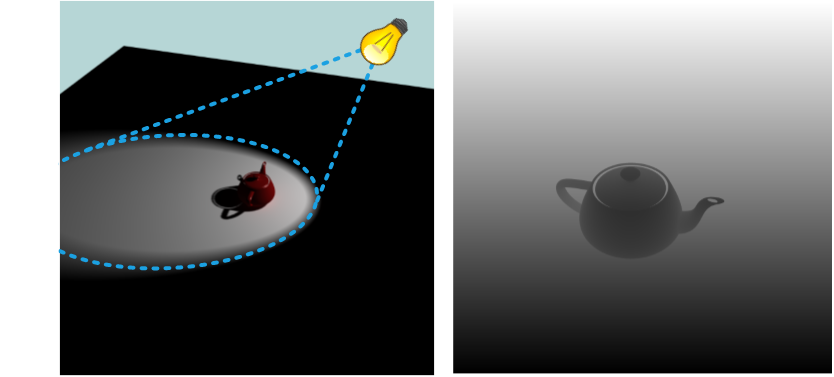
\includegraphics[width=1\textwidth]{res/img/shadow-mapping/shadow_map_principle.png}
    \caption{[Links] die Perspektive der Kamera mit eingezeichneter Lichtposition. 
    [Rechts] Die Tiefenwerte der Szene aus der Perspektive des Lichtes. 
    Diese Textur wird Shadow Map genannt.}
	\end{center}
	\label{fig:shadow-map}
\end{figure}
%arten von lichtquellen.
\section{Arten von Lichtquellen}
\label{section:types-of-sources}
Es gibt unterschiedliche Arten von Lichtern die sich alle mit Shadow Mapping darstellen lassen.
Das direktionales Licht ist ein Licht, bei dem alle Lichtstrahlen parallel verlaufen.
Dies lässt sich beim Shadow Mapping umsetzen, indem als Projektionsmatrix des Lichtes eine
Orthogonale Projektion verwendet wird.
Analog lässt sich ein Spot Light implementieren hier wird als Projektion eine Perspektivische Projektion verwendet.
Punkt Lichter können etwas komplizierter sein, doch wir wollen Punkt Lichter hier einfach als 6 Spotlights betrachten
die jeweils 90° abdecken dabei wird die Shadow Map in einer Würfel Textur mit 6 Seiten gespeichert.
Der Shadow Mapping Algorithmus verläuft für alle Lichter identisch nur die Wahl der Projektion wird verändert.

\section{Überblick der Diskretisierung Probleme}
\label{section:problem-overview}
Beinahe alle Probleme des Shadow Mapping Verfahren entstehen durch die Diskretisierung,
die gezwungenermaßen in Computern auftritt. 
Dabei tritt Diskretisierung in mehreren Dimensionen auf.
\newline \newline
Die erste Form der Diskretisierung die zu Fehlern führt ist die Werte-Diskretisierung 
in der Shadow Map. 
Bei dem Vergleich, ob ein Pixel im Schatten liegt oder von einer Lichtquelle beleuchtet wird,
kommt es zur falschen Klassifikation. Dieser Fehler entsteht durch runden der Tiefenwerte in der Shadow Map und
durch die numerische Instabilität der Lichttransformation.
Dies führt zu einem deutlich sichtbaren visuellen Artefakt, das Selbestverschattung genannt wird.
Selbestverschattung wird in Abschnitt \ref{section:self-shadow} genauer erklärt.
\newline \newline
Die zweite Dimension, in der Diskretisierungsfehler auftreten, ist die Pixel Auflösung der Shadow Map.
Diskretisierungsfehler die dadurch auftreten erzeugen Aliasing Artefakte.
Eine Möglichkeit diese zu verbessern funktioniert analog zu Geometrie Antialiasing, dabei kann jedoch
nicht die Shadow Map selbst gefiltert werden, sondern es werden die Vergleichsergebnisse gefiltert.
Dies führt dazu das die Schattenkanten geglättet werden. 
Eine mögliche Implementierung hiervon heißt Percentage Closer Filtering
und wird in Abschnitt \ref{section:pcf} behandelt.
\newline
\newline
Um andere Methoden zur Verbesserung des Aliasing Problems zu betrachten ist eine genauere Klassifikation des Aliasing Problems 
nötig. 
Dabei wird Aliasing in 2 Kategorien eingeteilt:
\begin{itemize}
  \item \textbf{Perspektive Aliasing} entsteht dadurch, dass Oberflächen die nahe bei der Kamera sind groß auf dem 
    Bildschirm dargestellt werden, jedoch wird für die Schattenberechnung dieselbe Anzahl an Shadow Map Pixeln verwendet,
    wie für Oberflächen, die sehr weit von der Kamera entfernt sind. 
    Der Effekt von Perspektive Aliasing ist maximal, wenn das Licht direkt in die Kamera leuchtet, denn hier 
    sind Oberfläche nahe bei der Kamera im Clip Space groß aber im Light Clip Space klein, 
    wodurch Oberflächen nahe bei der Kamera wenig Pixel auf der Shadow Map zugeordnet sind. 
    Dieses Szenario nennt man Duelling Frusta. 
    Analog ist der Effekt minimal, wenn die Lichtrichtung gleich der Sichtrichtung ist.
  \item \textbf{Projektives Aliasing} entsteht, wenn zwischen Pixeln in der Shadow Map und Pixeln 
    im Screen Space kein 1:1 Verhältnis existiert. Dieser Effekt ist besonders stark bei Oberflächen
    mit Normalen orthogonal zu der Lichtrichtung. Diese Oberflächen nehmen auf der Shadow Map nur sehr wenig 
    Pixel ein, wobei sie im Screen Space sehr groß sein können. 
\end{itemize}

\section{Selbestverschattung}
\label{section:self-shadow}
%erläuterung des Artefakts (mit Bild)
\begin{figure}[H]
	\begin{center}
    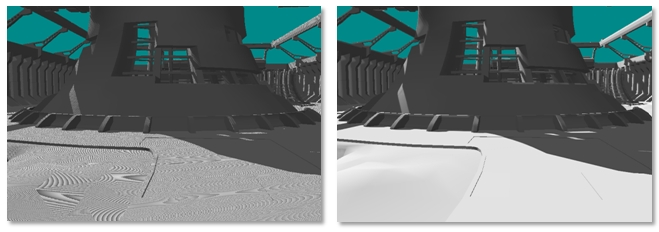
\includegraphics[width=1\textwidth]{res/img/shadow-acne1/image.jpg}
    \caption{Links\hspace{6}: Szene mit Selbstverschattung. 
         \newline Rechts: Szene ohne Selbstverschattung.
         \newline } 
	\end{center}
	\label{fig:shadow-acne-artefact}
\end{figure}
Selbstverschattung (Abbildung: \ref{fig:shadow-acne-artefact}) ist ein visuelles Artefakt.
Es tritt auf, wenn ein Punkt in der Shadow Map näher ist als tatsächlich, wodurch der Punkt sich selbst beschattet.
Dies kann an folgen Gründen liegen.
\begin{enumerate}
  \item Die Rundung der Tiefenwerte kann zu Selbestverschattung führen, dabei kann entweder der Tiefenwert in der Shadow Map
    abgerundet oder die Z-Komponente des Punktes in Light Clip Space aufgerundet worden sein.
  \item In der Shadow Map kann nicht die tatsächliche Tiefe eines Punktes
    gespeichert werden, sondern nur die Tiefe eines Bereichs, der von einem Pixel in der Shadow Map beschrieben wird.
    Für Oberflächen die parallel zur Lichtrichtung liegen und klein auf der Shadow Map dargestellt werden ist dieses Problem
    verstärkt.
\end{enumerate}


\begin{figure}[H]
	\begin{center}
    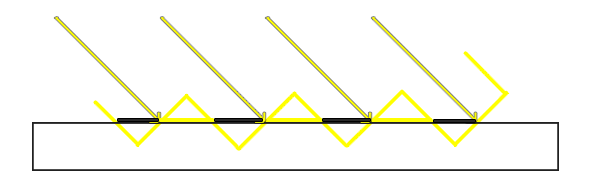
\includegraphics[width=1\textwidth]{res/img/shadow-acne3/image.png}
    \caption{Die Box ist ein beleuchtetes Objekt. 
      Die zackige gelbe Linie beschreibt die Tiefenwerte die tatsächlich in der Shadow Map gespeichert sind.
      Hier sind 2 Diskretisierungen zu bemerken; 
      die Breite der Shadow Map Pixel und der Höhenunterschied der Pixel (Tiefenauflösung).
      Der schwarze Teil der Box Oberfläche liegt im Licht, 
      da hier der Tiefenwert in der Shadow Map größer ist als der Abstand der Oberfläche zu dem Licht.
      analog liegt der gelbe Teil der Box Oberfläche im Schatten.
    }
	\end{center}
	\label{fig:shadow-acne-illu}
\end{figure}

Selbstverschattung kann durch einen Bias-Wert verringert werden.
Dabei wird vor dem Vergleich ein kleiner Wert (der Bias), auf den Tiefenwert in der Shadow Map addiert.
Bildlich kann man sich vorstellen, dass die gelbe gezackte Linie
(aus Abbildung: \ref{fig:shadow-acne-illu}) in die Lichtrichtung verschoben wird.
Es tritt keine Selbstverschattung mehr auf, wenn die komplette gelbe Linie unterhalb der Oberfläche liegt.
\newline \newline
Ein Konstanter Bias kann dabei helfen die Rundungsfehler (Grund: 1) zu verhindern.
Jedoch tritt weiterhin Selbstverschattung an Oberflächen auf die fast parallel zur Lichtrichtung liegen.
An diesen Oberflächen kann Selbstverschattung nur durch einen sehr großen Bias-Wert verhindert werden.
Dies führt jedoch zu einem Artefakt, dass Peter Panning heißt (Abbildung: \ref{fig:peter-panning}).
Dadurch das wir die Tiefenwerte der Shadow Map in Richtung des Lichtes mit einem Bias-Wert verschieben,
verschieben wir auch die Schatten selbst.
Dises Artefakt ist sehr unangenehm, den wie in Abschnitt \ref{ch:Introduction} erläutert, geben uns Schatten Informaitonen
über Skalierung und Position, wenn wir also Schatten verschieben dann führt das zu einer irreführenden Darstellung der Szene.

\begin{figure}[H]
	\begin{center}
    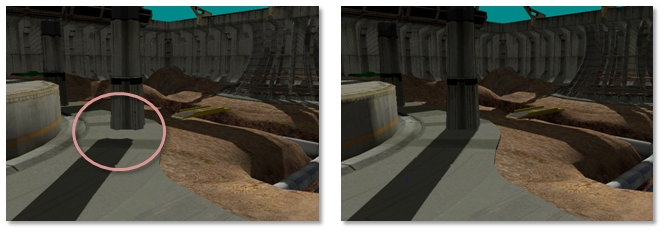
\includegraphics[width=1\textwidth]{res/img/peter-panning1/image.jpg}
    \caption{Links\hspace{6}: Szene mit Peter Panning Artefakt. Es führt oft dazu das es so scheint, als würden Objekte schweben.
        \newline Rechts: Szene ohne Peter Panning Artefakt.}
	\end{center}
	\label{fig:peter-panning}
\end{figure}

%einfache erläuterung von constant depth-bias.
%erläuterung von Peter panning (mit Bild)

\subsection{Heuristisches Biasing}
\label{section:heuristic-biasing}
Wie wir im letzten Kapitel gesehen haben kommt es ohne einen bias zu Selbestverschattung
und falls ein zu großer bias verwendet wird kommt es zu Peter-Panning.
Es sei außerdem zu bemerken, das bei Oberflächen die orthogonal zu der Lichtrichtung liegen 
ein nur sehr geringer bias benötigt wird, wobei für Oberflächen die parallel zu der Lichtrichtung 
liegen ein großer bias nötig ist.
Diese Beobachtung lässt sich ausnutzen indem der bias wert proportional zu dem sinus des Winkels zwischen
der Lichtrichtung und der Oberflächen Normalen gewählt wird.
Anstatt, den Winkel direkt auszurechnen, lässt sich dies effektiv mit dem Standard-Skalarprodukt berechnen.
Ein solcher bias wird Slope-Scale-Bias genannt.
Eine alternative Möglichkeit den proportionalen bias einzusetzen heißt Normal Offset Shadow Mapping.
Dabei wird die Oberfläche anstatt, in die Richtung des Lichtes, in die Richtung des Normalen Vektors 
verschoben.
\\
Beide dieser Verfahren verwenden die selbe Heuristik wobei die Stärke des bias 
proportional zu $1 - \overrightarrow{l} * \overrightarrow{n}$, wobei $\overrightarrow{l}$ 
die Lichtrichtung und $\overrightarrow{n}$ der Normalenvektor der Oberfläche ist.
Es sollte erwähnt werden, dass für Oberflächen die orthogonal zu der Lichtrichtung liegen
der heuristische bias 0 ist,
deshalb werden diese biasing Methoden oft mit einem konstanten bias kombiniert.
Das große Problem mit heuristischen biasing Methoden ist, dass 
diese für jede Szene neu konfiguriert werden müssen,
denn falls der bias zu groß ist so kommt es zu Peter-Panning und falls er zu klein gewählt 
wird kann es zu Selbestverschattung kommen.
Um die Konfiguration leichter zu machen werden oft Kombinationen 
von unterschiedlichen biasing Methoden verwendet wie zum Beispiel : \\
Slope-Scale-Bias + Normal-Offset-Shadow-Mapping + Konstanter Bias.
%TODO WHY DOES NORMAL OFFSET SHADOW MAPPING WORK.
\subsection{Alternative Techniken}
\label{section:sdsm}
Eine Alternative zu einem bias Wert heißt Second Depth Shadow Mapping.
Dieses funktioniert jedoch nur für Scenen mit solider Geometrie.
Dabei wird in der Shadow Map anstatt der Geometrie die am nähesten zum 
Licht ist, die Geometrie abgespeichert die am zweit nähesten zum Licht ist.
Dies lässt sich effektiv implementieren, indem anstatt von Back Face Culling, Front Face Culling verwendet wird.
Dadurch kommt es zu keiner Selbestverschattung mehr, da die Oberfläche die am nähsten an der 
Lichtquelle liegt immer im Licht ist, denn beim Vergleich der Tiefenwerte werden
keine zwei Werte verglichen, die nah beieinander liegen.
Es könnte jedoch Selbestverschattung auf der Rückseite der Geometrie auftreten.
Da die Geometrie solide ist, kann für Oberflächen die von dem Licht wegzeigen direkt 
angenommen werden das sie im Schatten liegen.
Außerdem tritt kein Peter-Panning auf, da kein bias verwendet wird.
Doch wie bereits erwähnt erfordert Second Depth Shadow Mapping, das die
Geometrie der Szene solide ist.
Doch auch mit solider Geometrie kann Selbestverschattung auftreten.
Wenn die Geometrie sehr dünn ist dann, dann ist der Tiefenunterschied zwischen Front und Back Face zu gering, 
wodurch beim Vergleich wieder Selbstverschattung auftritt.
\section{Bestimmen eines engen Licht Frustums}
\label{section:fit-the-frustum}
Alle Probleme die im letzten Kapitel besprochen wurden, sowie fast alle
diskretisierungs Probleme die beim Shadow Mapping auftreten, können
durch eine höhere Auflösung der Tiefe oder eine höhere Anzahl an Pixeln in der Shadow Map verbessert werden.
Da dies jedoch oft nicht möglich ist, kann stattdessen die effektive Auflösung verbessert werden.
Dies basiert auf der Beobachtung, das nur Objekte die Schatten werfen,
die von der Kamera sichtbar sind, in der Shadow Map gezeichnet werden müssen.
Um die effektive Auflösung zu verbessert können wir das Licht Frustum 
so wählen, das die 4 Punkte erfüllt sind (Abbildung: \ref{fig:fit-the-frustum})
\begin{enumerate}
  \item Die Größe des Lichtfrustums ist minimal.
  \item Die Form des Lichtfrustums stimmt mit der Art des Lichtes überein.
  \item Alle Punkte die im Kamera Frustum enthalten sind, sind auch im Licht Frustum enthalten.
  \item Alle Punkte die potentiel Schatten werfen können sind im Licht Frustum enthalten.
\end{enumerate}
Dadurch das die Form und die Richtung des Lichtfrustums beibehalten werden muss,
kann nur die Distanz zwischen Near und Far Plane angepasst werden.
Je kleiner der Abstand zwischen Near und Far Plane, desto besser 
ist die effektive Auflösung.
Das bedeutet das Near und Far Plane so gewählt werden müssen, das die Near Plane
möglichst groß ist und die Far Plane möglichst klein.
Dies können wir berechnen, indem wir zuerst die Eckpunkte des Kamerafrustums 
in das Lichtkoordinatensystem bringen um anschließend 
die minimale und maximale z-Koordinate der Punkte zu betrachten.
Die minimale z-Koordinate wählen wir als Near Plane.
Die maximale z-Koordinate wählen wir als Far Plane.
Es ist jedoch zu bemerken, dass Punkte die nicht im Kamerafrustum liegen
auch Schatten werfen können. 
Um dies zu ermöglichen kann die Near Plane nach hinten verschoben werden
um Punkte zu enthalten, die außerhalb des Kamerafrustums liegen, aber trotzdem Schatten werfen können.
\newline \newline
Für direktionale Lichter wie die Sonne ist dieses Verfahren besonders wichtig,
denn eine Shadow Map die alle Objekte der Szene enthalten würden,
würden viele unnötige Tiefen Information besitzen die nicht verwendet wird.
Außerdem kann dieses Verfahren leicht angepasst werden, um die Position des Lichtfrustums 
zu verändern, wodurch es unmöglich wird die Kamera an eine Stelle zu bewegen, an der das 
direktionale Licht keine Schatten mehr wirft, da sich das Lichtfrustum mit dem Kamerafrustum mitbewegt.

\begin{figure}
	\begin{center}
		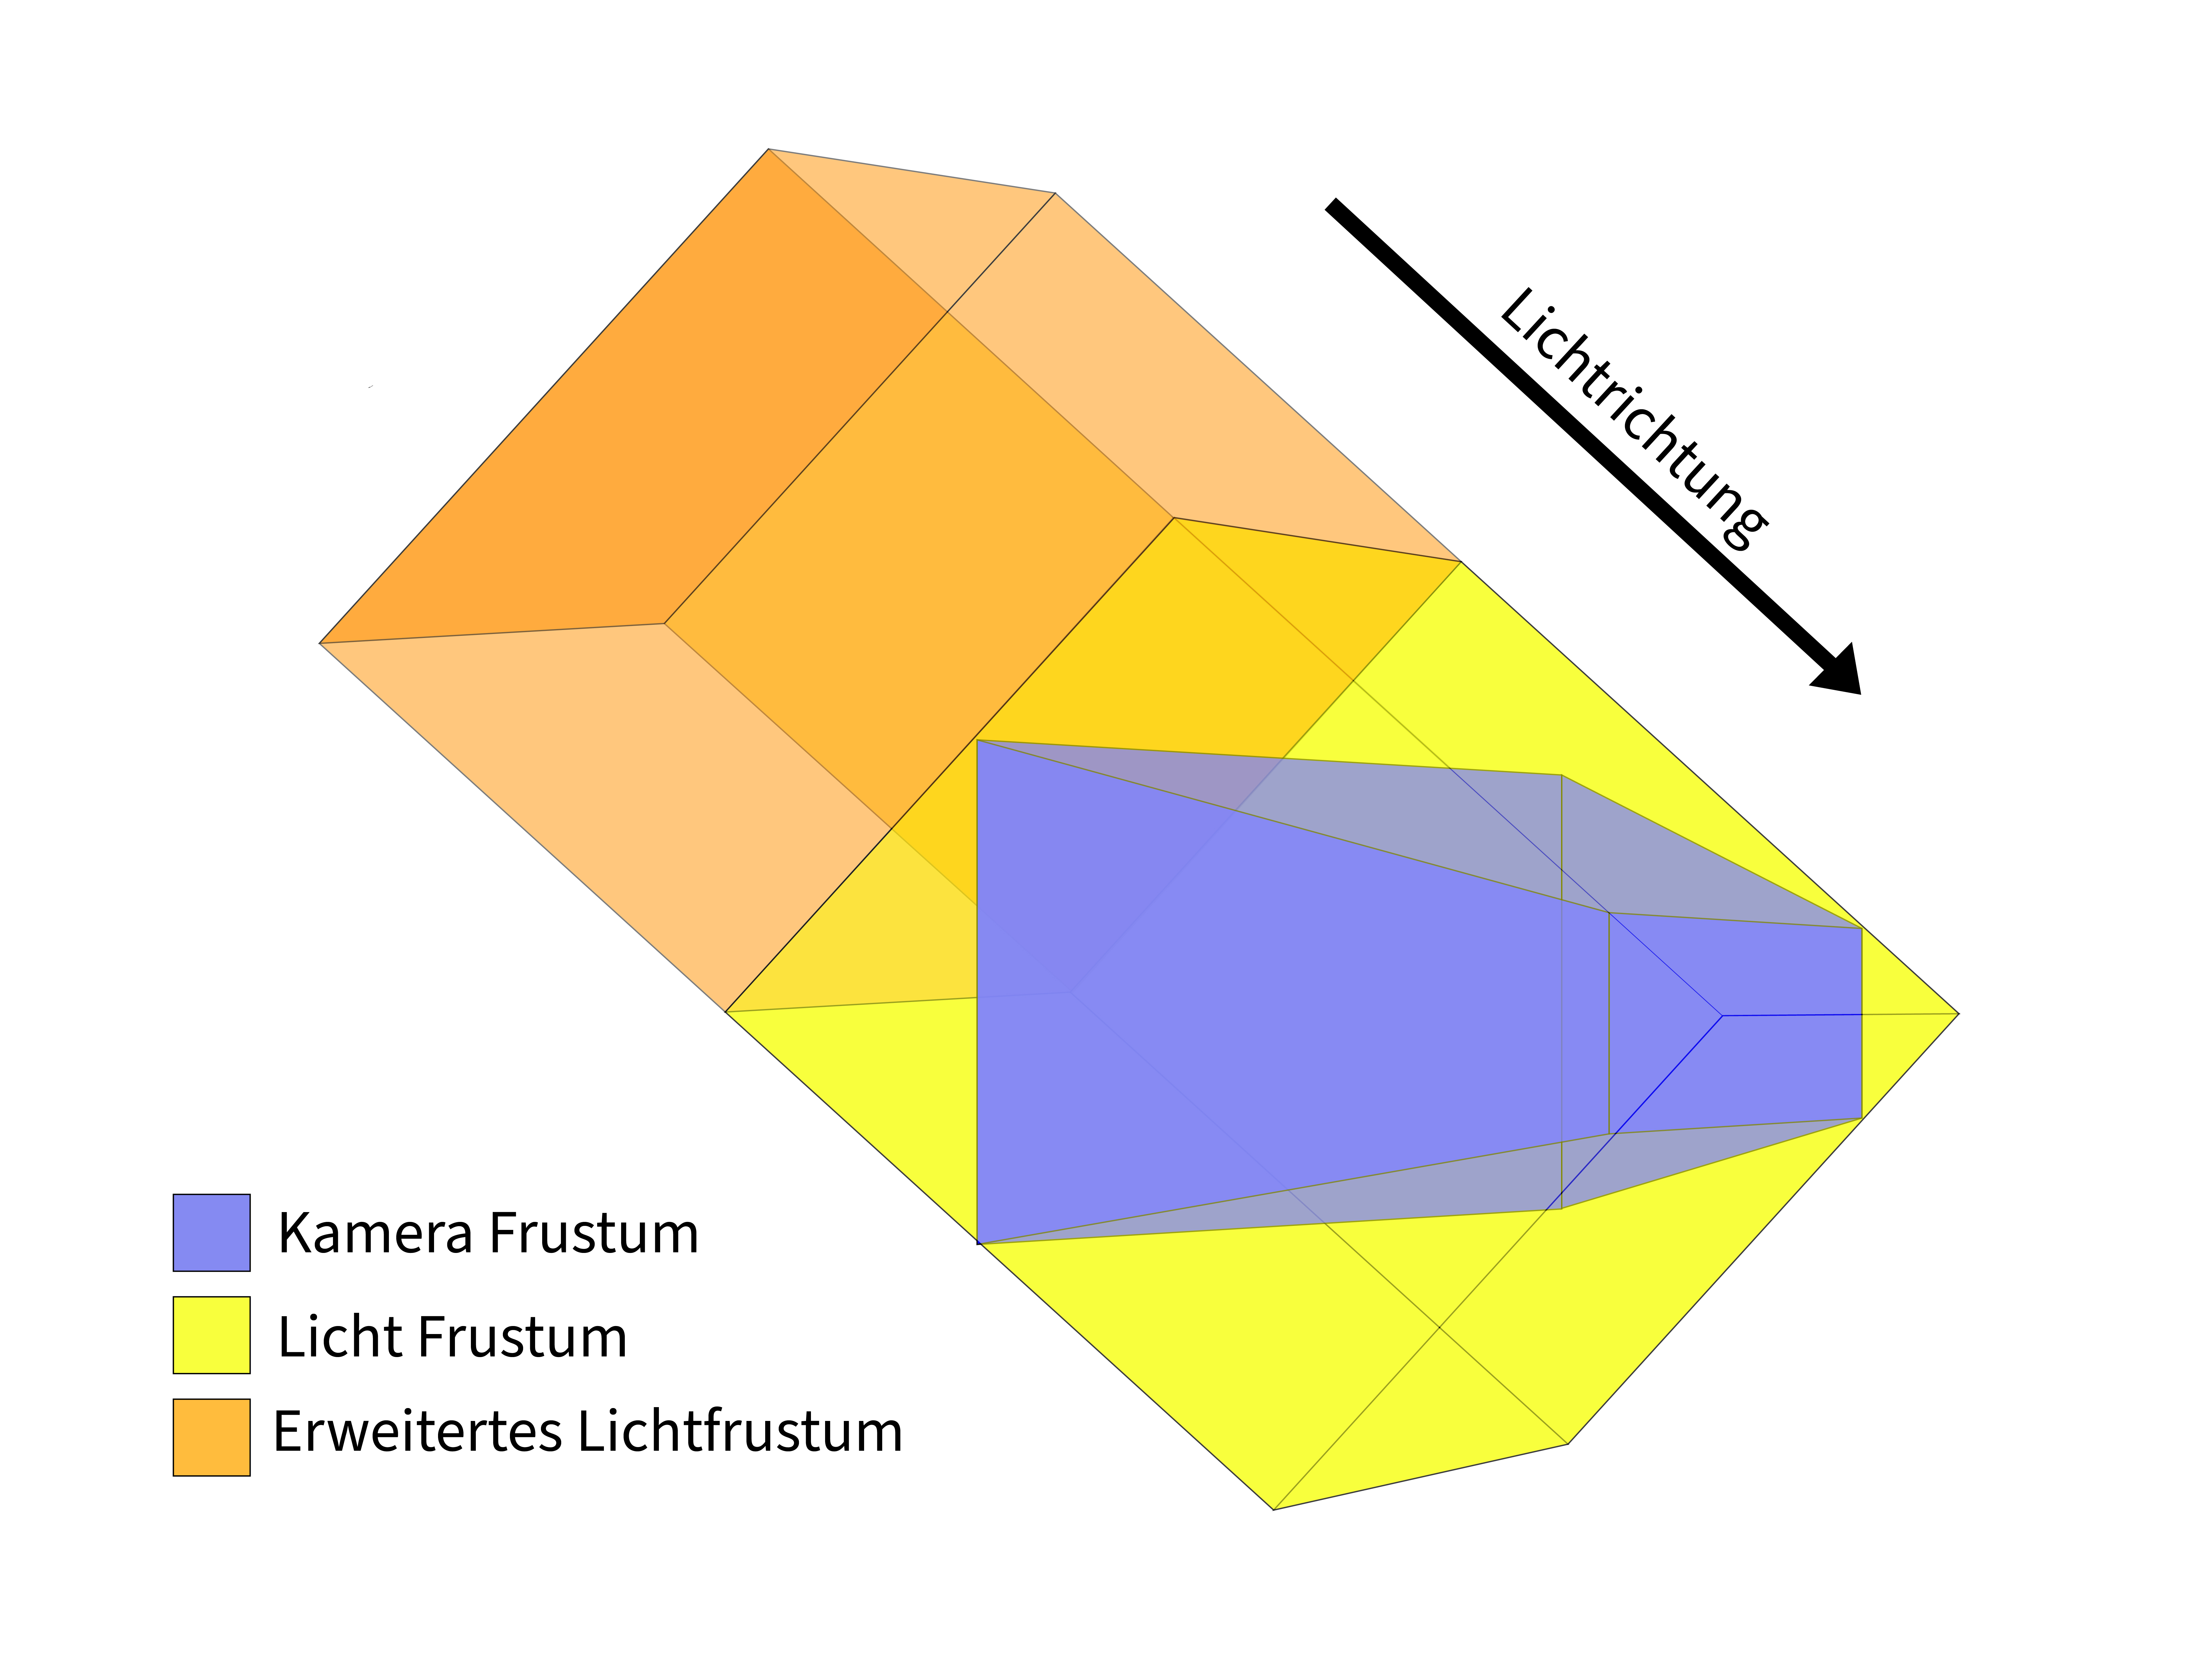
\includegraphics[width=1\textwidth]{res/img/fit-the-frustum.jpg}
    \caption{}
	\end{center}
	\label{fig:fit-the-frustum}
\end{figure}
\section{Perspektivisches Aliasing}
\label{section:perspective-aliasing}
Perspektivisches Aliasing entsteht wie der Name schon andeutet durch die Perspektivische Projektion
der Kamera. Das bedeutet, das Punkte die näher an der Kamera sind größer auf dem Bildschirm dargestellt werden.
Perspektivisches Aliasing entsteht nun dadurch das dieses Verhältnis für die Shadow Map nicht gilt.
Das bedeutet, das ein Punkt, der sehr nah an der Kamera ist und deshalb sehr groß dargestellt wird,
in der Shadow Map gleich groß ist wie ein Punkt der aus der Perspektive der Kamera sehr klein ist.
Dies führt dazu das bei Oberflächen die nahe an der Kamera liegen die einzelnen Pixel der Shadow Map klar erkennbar sind (Abbildung: \ref{fig:perspective-aliasing}).
\begin{figure}
	\begin{center}
		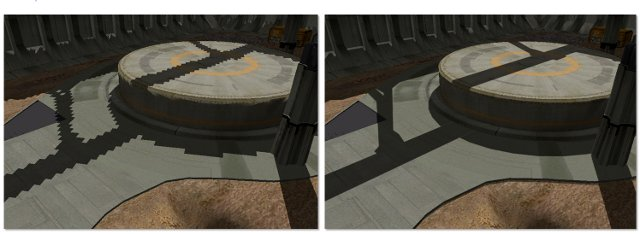
\includegraphics[width=1\textwidth]{res/img/perspective-aliasing1/image.jpg}
    \caption{}
	\end{center}
	\label{fig:perspective-aliasing}
\end{figure}
\subsection{Perspective Shadow Mapping}
\label{section:psm}
Eine Möglichkeit um Perspektivisches Aliasing zu verhindern ist das verzerren 
des Shadow Map Koordinatensystems. 
Dabei wird das Koordinatensystem so verzerrt, dass Oberflächen die nahe an der Kamera liegen in dem
Lichtkoordinatensystem größer sind und dadurch eine höhere Auflösung haben.
Eine mögliche Implementierung davon heißt Perspective Shadow Mapping (PSM) \cite{PSM2002}.
Hier wird das Lichtkoordinatensystem mit der Kameratransformation selbst transformiert, wodurch
die Perspektive der Kamera ebenfalls auf das Lichtkoordinatensystem angewendet wird.
Dadurch ist das Perspektive Aliasing uniform auf alle Pixel verteilt,
wodurch der Einfluss auf die visuelle Qualität minimiert wird.
Dieses Verfahren kommt jedoch mit einigen Problemen:
\begin{itemize}
  \item Die Schattenberechnung wird nun in Post Perspective Space durchgeführt (auch Normalized Device Space genannt).
    Hier müssen Direktionale Lichter als Punkt Lichter und Punkt Lichter als Direktionale Lichter interpretiert werden.
    Das führt dazu, dass das bildliche Denken in diesem Raum sehr schwierig ist.
  \item Es tritt weiterhin Projektives Aliasing.
\end{itemize}
Eine Verbesserung von PSM heißt Light Space Perspective Shadow Mapping (LiSPSM) \cite{LiPSM2004}.
Hier wird anstatt der Kameratransformation der Raum mit einer einfacheren Verzerrungsmatrix transformiert.
Dadurch kann ebenfalls Perspektivisches Aliasing verhindert werden und
durch die einfachere Wahl der Matrix muss die Schattenberechnung zwar immernoch im Post Perspective Space durchgeführt werden,
aber jetzt bleiben Direktionale Lichter, Direktionale Lichter.
Die Stärke der Verzerrung hängt nun von einem Parameter $n$ ab. 
In dem gleichen Paper in dem LiSPSM vorgestellt wurde, wird ebenfalls eine optimale Wahl für $n$ berechnet
die Projektives Aliasing minimiert : $n_{opt} = near + \sqrt{near * far}$.
LiSPSM entfernt demnach Perspektivisches Aliasing und auch Projektives Aliasing kann durch LiSPSM in vielen Fällen
minimiert werden.
\subsection{Cascaded Shadow Mapping}
\label{section:csm}
TODO find original PAPER that introduced CSM.\\
Cascaded Shadow Mapping (CSM) ist ein weiteres Verfahren um Perspektives Aliasing zu vermeiden.
Im Vergleich zu LiSPSM wird der Raum bei CSM nicht verzerrt, sondern in $N$ Räume partitioniert (Abbildung X.Y).
\newline
Der Algorithmus lässt sich in folge Schritte unterteilen:
\begin{enumerate}
  \item Partitioniere das View Frustum in N Räume. 
    Teile dafür das View Frustum an N Oberflächen die orthogonal zu der Near und Far Plane liegen.
    Eine Möglichkeit diese Flächen zu verteilen ist exponentiel : $z_{i} = N * (far / near)^{i/N}$
  \item Berechne eine enge Projektion [\ref{section:fit-the-frustum}] um jede Partition des View Frustums.
    Zeichne anschließend die Szene mit den $N$ berechneten Projektionen.
    Die $N$ erzeugeten Shadow Maps heißen Kaskaden.
  \item Zeichne die Szene aus der Kamera Perspektive. 
    Die Schatten berechnung muss dabei leicht angepasst werden.
    Bei dem Vergleich, im Shadow Mapping Algorithmus, muss jetzt der Tiefenwert mit allen Kaskaden verglichen werden.
\end{enumerate}
Es ist zu bemerken, dass CSM eine Diskretisierung von LiSPSM, denn falls $N\rightarrow\infty$ sind beide Verfahren identisch. 
Durch die Diskretisierung kommt es dazu das der Übergang zwischen Kaskaden oft sichtbar ist.
Es ist Möglich LiSPSM zu verwenden um die einzelnen Kaskaden zu zeichnen, doch dies führt dazu das die Schattenberechnung wieder
in Post Perspektive Space durchgeführt wird. 
Eine andere Möglichkeit ohne die Form des Lichtfrustums zu verändern ist eine andere Verteilung der Kaskaden\\
$z_{i} = \lambda{}N(far/near)^{i/N} + (1-\lambda{})(n+(i/near)(far - near)$\\
Dabei ist $\lambda$ ein Faktor, der die Stärke der Korrektion vorgibt.
\newline \newline
Der Große Vorteil von CSM ist, dass die berechnung der Schatten nicht in Post Perspective Space wie bei PSM oder LiSPSM 
durchgeführt wird. 
Dadurch können Punkt Lichter als Punkt Lichter und Direktionale Lichter als Direktionale Lichter behandelt werden.
CSM eignet sich außerdem für große Lichtquellen wie beispielsweise die Sonne, die die gesamte Szene beleuchten.
Solche Lichter benötigen eine hohe Auflösung und da die Auflösung in CSM auf $N$ Texturen aufgeteilt wird können hierfür beispielsweise 
4x 4000x4000 Texturen verwendet werden. Diese Auflösung ist mit LiSPSM nicht möglich da viele Grafikkarten keine
16000x16000 Texturen unterstützen.
Es sollte jedoch bei CSM nicht vergessen werden, das es Perspektivisches Aliasing nicht so gut entfernt, wie 
LiSPSM, da CSM eine Diskretisierung von LiSPSM ist.
In der Praxis ist die Diskretisierung von CSM jedoch selten erkennbar, weshalb CSM verbreiteter wie LiSPSM ist \cite{Survey2011}.

\section{Projektives Aliasing}
\label{section:projective-aliasing}
Projektives Aliasing entsteht dadurch, dass die Pixel der Kamera nicht in 
einem 1:1 Verhältnis zu den Pixeln in der Shadow Map stehen (Abbildung: \ref{fig:projective-aliasing}).
\begin{figure}
	\begin{center}
		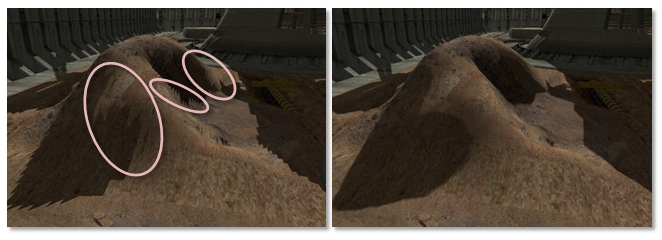
\includegraphics[width=1\textwidth]{res/img/projective-aliasing/image.jpg}
    \caption{}
	\end{center}
	\label{fig:projective-aliasing}
\end{figure}
\newline \newline
Die meisten Verfahren die auch Perspektivisches Aliasing verbessern helfen auch dabei Projektives Aliasing zu vermeiden.
Dies liegt daran, dass diese Verfahren die effektive Auflösung der Shadow Map verbessern.
Projektives Aliasing ist besonders stark, wenn die Lichtrichtung orthogonal zu der Sichtrichtung ist.
In diesem Fall helfen Verfahren die Projektives Aliasing entfernen nicht mehr.
Die einzigste Möglichkeit um nun Projektives Aliasing zu entfernen scheint das Erhöhen der Auflösung zu sein.
\section{Percentage Closer Filtering}
\label{section:pcf}
Percentage Closer Filtering kann Projektives Aliasing verbessern ohne dabei die Auflösung der Shadow Map zu steigern, 
doch das ist nicht die Hauptfunktion davon.
Percentage Closer Filtering bekämpft ein Grundlegenderes Problem.
Die einzelnen Pixel der Shadow Map sind klar in der Szene erkennbar.

Dieses Problem lässt sich mit Geometrie Aliasing vergleichen hier sind die Stufen der Geometrie eindeutig erkennbar,
obwohl die zu grundeliegende Geometrie kontinuierlich ist (Abbildung: \ref{fig:pixel-aliasing}). 
Das Problem lässt sich Verbessern, indem Pixel nicht binär in 2 Klassen eingeteilt werden 
(gehört zur Geometrie oder gehört nicht zur Geometrie), sondern partiell zur Geometrie gehören können (Der Pixel gehört zu 20\% zur Geometrie).
\begin{figure}
	\begin{center}
		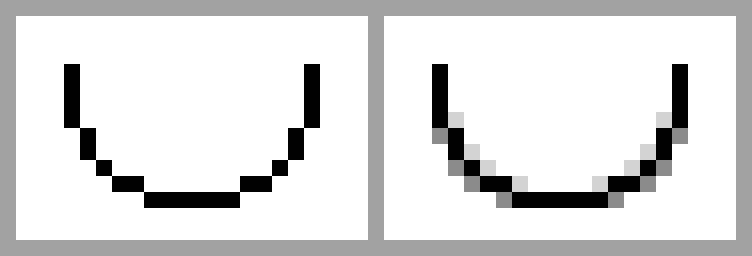
\includegraphics[width=0.5\textwidth]{res/img/pixel-aliasing/image.png}
    \caption{}
	\end{center}
	\label{fig:pixel-aliasing}
\end{figure}
\newline \newline
Das gleiche Prinzip lässt sich auch auf Shadow Maps anwenden.
Dabei wird jeder Vergleich in dem Shadow Mapping Algorithmus mit den 4 nächsten Pixeln durchgeführt,
um anschließend partiell zu Klassifizieren wie sehr der Pixel im Schatten liegt.
Dies führt dazu das die Schattenkanten weicher gezeichnet werden. 
Es sollte jedoch bemerkt werden, dass dies nicht mit Soft Shadows zu vergleichen ist, 
in mancher Literatur werden solche Verfahren als Psudo Soft Shadows bezeichnet, denn sie 
zeichnen alle Schattenkanten gleich weich.
\section{Variance Shadow Mapping}
\label{section:vsm}
TODO explain VSM and compare it to PCF.

\chapter{Fazit}
Das schreibe ich am Ende. Aktuell würde ich ehrlich gesagt noch gerne auf VSH eingehen,
weil PCF ja nicht wirklich Echtzeitfähig ist und
ich würde gerne eine Echtzeitfähige Kombination von Algorithmen vorstellen.

















